\documentclass[a4paper,12pt]{article} %размер бумаги устанавливаем А4, шрифт 12пунктов
\usepackage[utf8]{inputenc}
\usepackage{csquotes}
\usepackage[english,russian]{babel}%используем русский и английский языки с переносами
\usepackage{biblatex}
\bibliography{refs}
\usepackage{amssymb,amsfonts,mathtext,enumerate,float} %подключаем нужные пакеты расширений
\usepackage{textcomp}
\usepackage{adjustbox}
\usepackage{graphicx} %хотим вставлять в диплом рисунки?
\makeatletter
\makeatother
\usepackage{sagetex}
\usepackage{geometry} % Меняем поля страницы
\geometry{left=2cm}% левое поле
\geometry{right=1.5cm}% правое поле
\geometry{top=1cm}% верхнее поле
\geometry{bottom=2cm}% нижнее поле
\usepackage{tabularx}
\usepackage{threeparttable}
\usepackage{epstopdf}
\usepackage{amsmath} %отображение математической нотации
\usepackage{caption, subcaption} %подписи}
\usepackage{indentfirst}%отступ вначале параграфа
\usepackage{pscyr}

\captionsetup[table]{labelsep = endash, singlelinecheck=false}
\captionsetup[figure]{name = Рисунок, labelformat=simple, labelsep = endash}



\begin{document}


\newcommand\tline[2]{$\underset{\text{#1}}{\text{\underline{\hspace{#2}}}}$}
\newcommand\nameLine[3]{$\underset{\text{#1}}{\text{\underline{\text{#2}\hspace{#3}}}}$}

\begin{titlepage}
	\centering
	{\fontsize{12pt}{5cm}\selectfont \bfseries Министерство образования и науки Российской Федерации} \\ \vspace{0.5cm}
	{\fontsize{7pt}{5cm}\selectfont ФЕДЕРАЛЬНОЕ ГОСУДАРСТВЕННОЕ АВТОНОМНОЕ ОБРАЗОВАТЕЛЬНОЕ УЧРЕЖДЕНИЕ ВЫСШЕГО ПРОФЕССИОНАЛЬНОГО ОБРАЗОВАНИЯ} \\ 
	\vspace{1cm}
	{\fontsize{12pt}{5cm}\selectfont \bfseries САНКТ-ПЕТЕРБУРГСКИЙ УНИВЕРСИТЕТ ИНФОРМАЦИОННЫХ ТЕХНОЛОГИЙ, МЕХАНИКИ И ОПТИКИ} \\ \vspace{1.5cm}
	
	{\fontsize{14pt}{5cm}\selectfont Кафедра \hspace{1cm} \underline{Систем Управления и Информатики}  \hspace{1cm} Группа \underline{Р3340}} \\
	
	\vspace{2cm}
	
	{\fontsize{20pt}{5cm}\selectfont \bfseries Лабораторная работа №9} \\
	{\fontsize{20pt}{5cm}\selectfont \bfseries “Экспериментальное построение частотных характеристик типовых динамических звеньев”} \\
	\vspace{0.2cm}
	{\fontsize{14pt}{5cm}\selectfont Вариант - 10} \\
	
	\vspace{1.5cm}
	
	\flushleft
	{Выполнилa \hspace{1.8cm} \nameLine{(фамилия, и.о.)}{Ким А. А.}{7cm} (подпись)} \\
	
	\vspace{2cm}
	
	{Проверил \hspace{2cm} \tline{(фамилия, и.о.)}{9cm} (подпись)} \\
	
	\vspace{5cm}
	
	"\underline{\hspace{0.7cm}}"\hspace{0.2cm}\underline{\hspace{2cm}}\hspace{0.2cm}20\underline{\hspace{0.7cm}}г. \hspace{2cm} Санкт-Петербург, \hspace{2cm} 20\underline{\hspace{0.7cm}}г. \\ \vspace{1cm}
	
	Работа выполнена с оценкой \hspace{1cm} \underline{\hspace{8cm}} \\ 
	\vspace{1cm}
	Дата защиты "\underline{\hspace{0.7cm}}"\hspace{0.2cm}\underline{\hspace{2cm}}\hspace{0.2cm}20\underline{\hspace{0.7cm}}г.
\end{titlepage}
\setcounter{page}{2}

\paragraph{Цель работы:}Исследование динамических и частотных характеристик, анализ структурных свойств и устойчивости линейных непрерывных систем с помощью прикладного пакета Matlab Control System Toolbox.
\paragraph{Исходные данные.}
Исходная модель разомкнутой системы представляется в форме вход-выход и
описывается передаточной функцией вида:
\begin{equation} 
W(s) = \frac{b_1s+b_0}{s\cdot(a_2s^2+a_1s+a_0)}.
\end{equation}

Значения коэффициентов $a_0, a_1, a_2, b_0, b_1$ в числителе и знаменателе передаточной функции для выполнения лабораторной работы выбираются самостоятельно произвольно из условия $a_2\neq0, b_1\neq0$.\par 
Выбранные значения коэффициентов: $a_0=6, a_1=6, a_2=6, b_0=5, b_1=-1$.
Тогда передаточная функция будет выглядеть следующим образом:
\begin{equation} 
W(s) = \frac{5s-1}{s\cdot(6s^2+6s+6)}.
\end{equation}

\newpage
\section{Анализ исходной разомкнутой системы}
Получим представление исходной системы в виде передаточной функции.
\begin{equation} 
W(s) = \frac{5s-1}{6s^3+6s^2+6s}.
\end{equation}

Найдём нули и полюса передаточной функции разомкнутой системы, результат представим в виде графика (рисунок \ref{pzmap}).\par
Нули передаточной функции --- корни числителя, полюса --- корни характеристического уравнения знаменателя. Исходя из этого $p_1=0+j0, p_2=-0.5+j0,8660, p_3=-0.5-j0,8660, z=0,2+j0$, где z---ноль.
\begin{figure}[ht!]
	\centering
	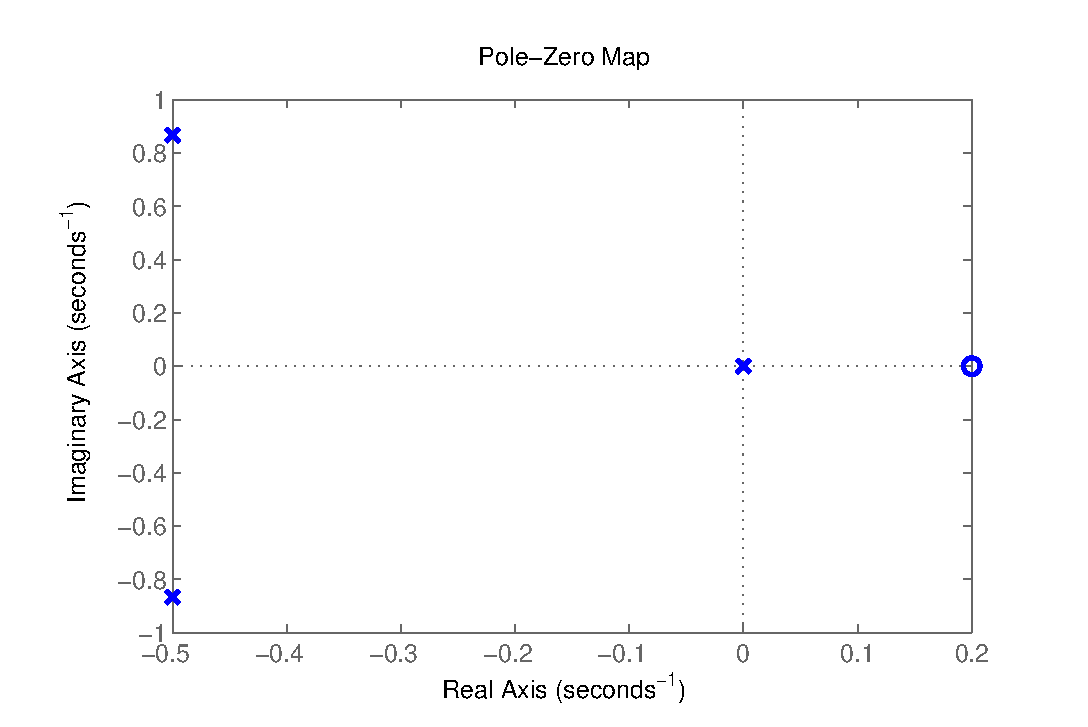
\includegraphics[width=1\linewidth]{scheme/pzmap}
	\caption{Нули и полюса системы}
	\label{pzmap}
\end{figure}\par
Для определения устойчивости системы обратимся к корневому критерию, в соответствии с которым система находится на нейтральной границе устойчивости, так как имеет чисто нулевой полюс и не имеет полюсов с положительной вещественной частью, что видно на рисунке \ref{pzmap}.

Получим графики логарифмических амплитудно-частотной и фазочастотной характеристик (рисунок \ref{bode}).\par
По графика на рисунке \ref{bode} видно, что частота среза равна 0,706 рад/с, запас устойчивости системы по амплитуде бесконечный, по фазе равен 141 градуса.
\begin{figure}[H]
	\centering
	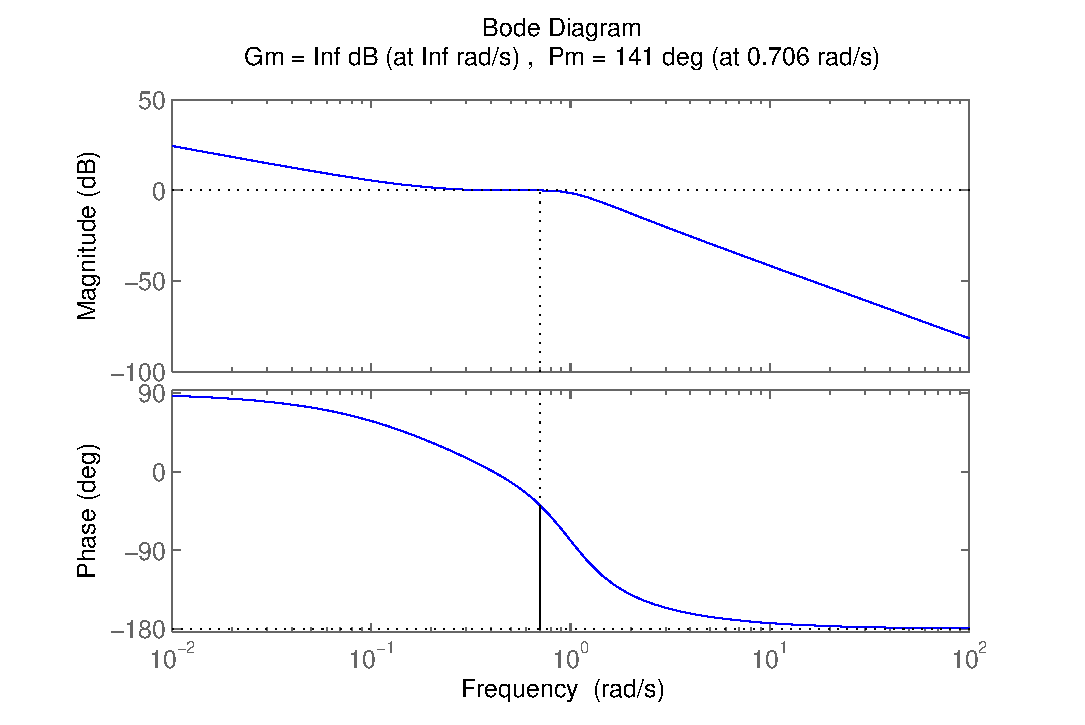
\includegraphics[width=0.9\linewidth]{scheme/bode}
	\caption{Логарифмические частотные характеристики системы}
	\label{bode}
\end{figure}

Построим амплитудно-фазочастотную характеристику исходной системы (рисунок \ref{nyquist}).\par
\begin{figure}[H]
	\centering
	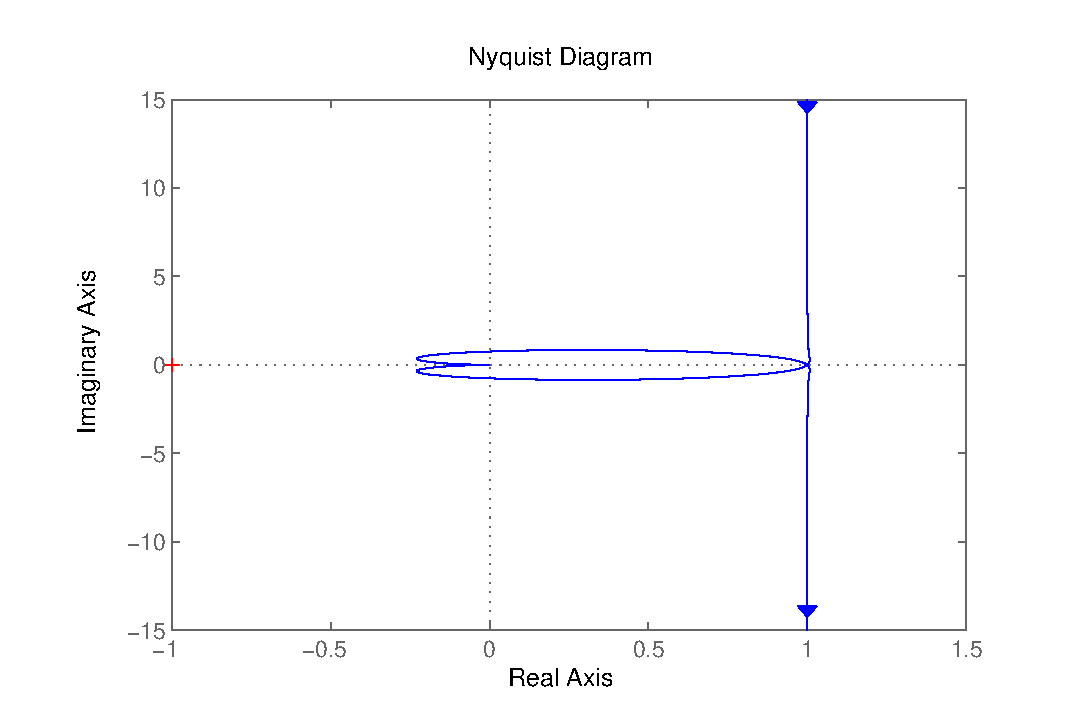
\includegraphics[width=0.9\linewidth]{scheme/nyquist}
	\caption{АФЧХ исследуемой системы}
	\label{nyquist}
\end{figure}
На графике \ref{nyquist} видно, что АФЧХ системы не охватывает точку (-1; j0). Следовательно, система является устойчивой по критерию Найквиста.

\newpage
\section{Анализ замкнутой системы}
Передаточная функция системы с жесткой отрицательной обратной связью в общем случае будет иметь вид:
\begin{equation}
\Phi(s) = \frac{\displaystyle{\frac{5s - 1}{6s^3 + 6s^2 + 6s}}}{1 + \displaystyle{\frac{5s - 1}{6s^3 + 6s^2 + 6s}}\cdot K} = \frac{5s - 1}{6s^3 + 6s^2 + (6 + 5K)s - K}
\end{equation}\par
Анализ влияния коэффициентов отрицательной обратной связи на расположение полюсов замкнутой системы представим в виде графика на рисунке \ref{rlocus}.
\begin{figure}[H]
	\centering
	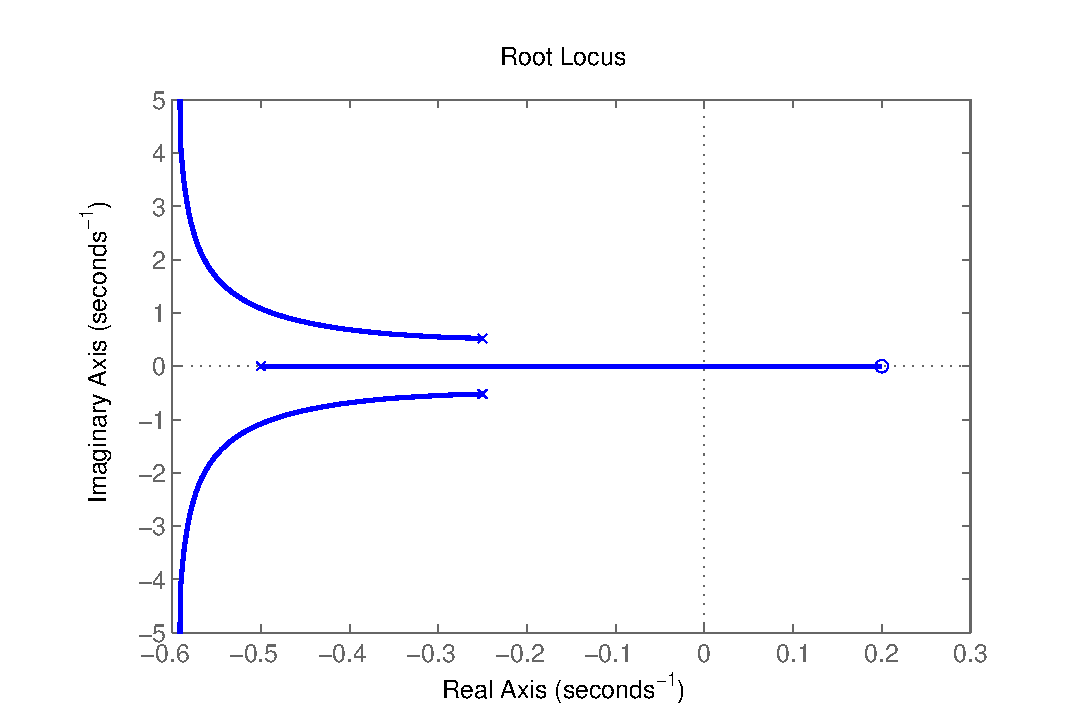
\includegraphics[width = 1\textwidth]{scheme/rlocus}
	\caption{Зависимость расположения полюсов замкнутой системы от коэффициента обратной связи}
	\label{rlocus}
\end{figure}
Для выбора коэффициента К воспользуемся корневым критерием устойчивости и составим матрицу Гурвица:
\[
\begin{vmatrix}
6 & -K & 0\\
6 & 6+5K & 0\\
0 & 6 & -K
\end{vmatrix}
\]
откуда видно, что при $K = 0$ система будет находиться на нейтральной границе устойчивости, при $K = -1$ --- находиться на колебательной границе устойчивости, при $K \in (-1;0)$ --- устойчива.
	
Выберем коэффициент обратной связи $K = -0,5$ тогда передаточная функция замкнутой системы примет вид
\begin{equation}
\Phi(s) = \frac{5s - 1}{6s^3 + 6s^2 + 3,5s + 1}.
\end{equation}

Найдём нули и полюса передаточной функции замкнутой системы, результат представим в виде графика (рисунок \ref{pzmap2}).\par
Исходя из графика $p_1=-0,5+j0, p_2=-0,25+j0,5204, p_3=-0,25-j0,5204, z=0,2+j0$, где z---ноль.
\begin{figure}[ht!]
	\centering
	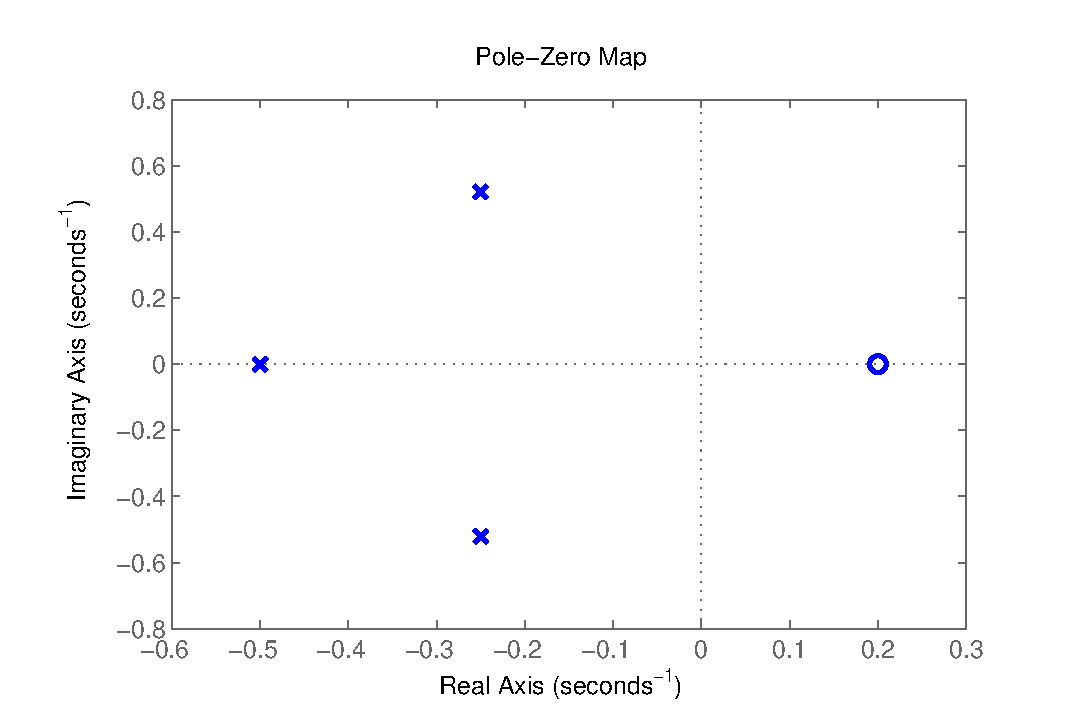
\includegraphics[width=1\linewidth]{scheme/pzmap2}
	\caption{Нули и полюса замкнутой системы}
	\label{pzmap2}
\end{figure}\par

Система устойчива, так как не имеет корней с неотрицательной вещественной частью.

Построим графики переходной и весовой функций замкнутой системы, изобразим полученные графики на рисунке \ref{stepimpulse}.
\begin{figure}[H]
	\centering
	\begin{subfigure}[b]{0.48\textwidth}
	    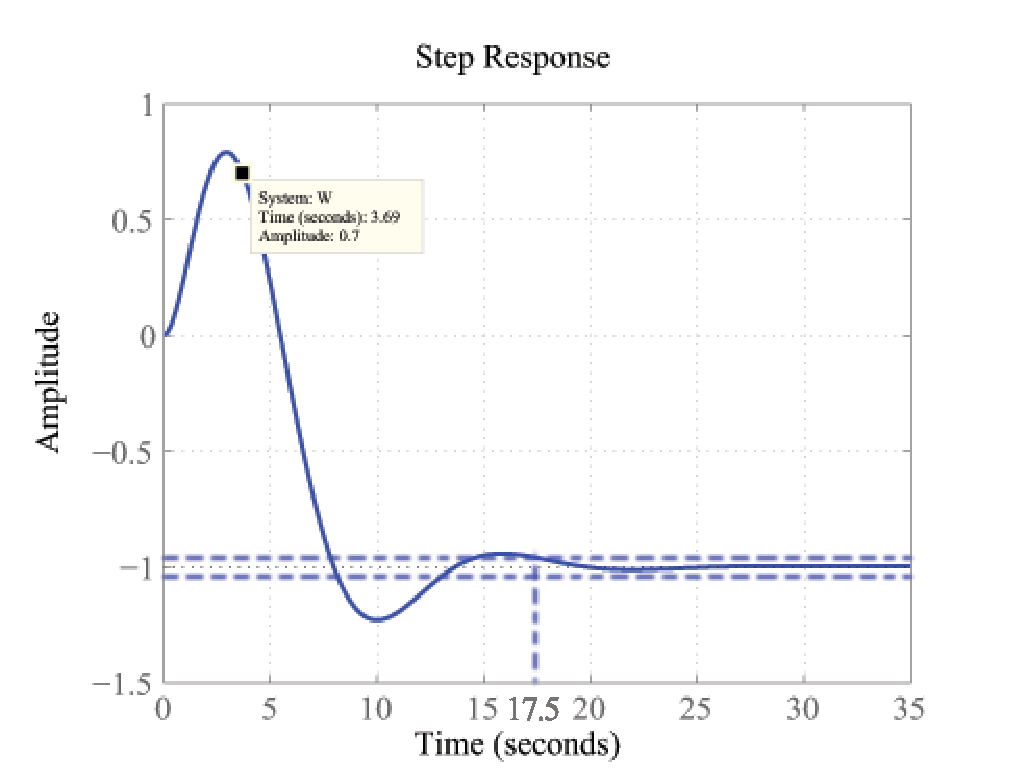
\includegraphics[width = \textwidth]{scheme/step}
		\caption{График переходной функции}
	\end{subfigure}
	\hfill
	\begin{subfigure}[b]{0.48\textwidth}
		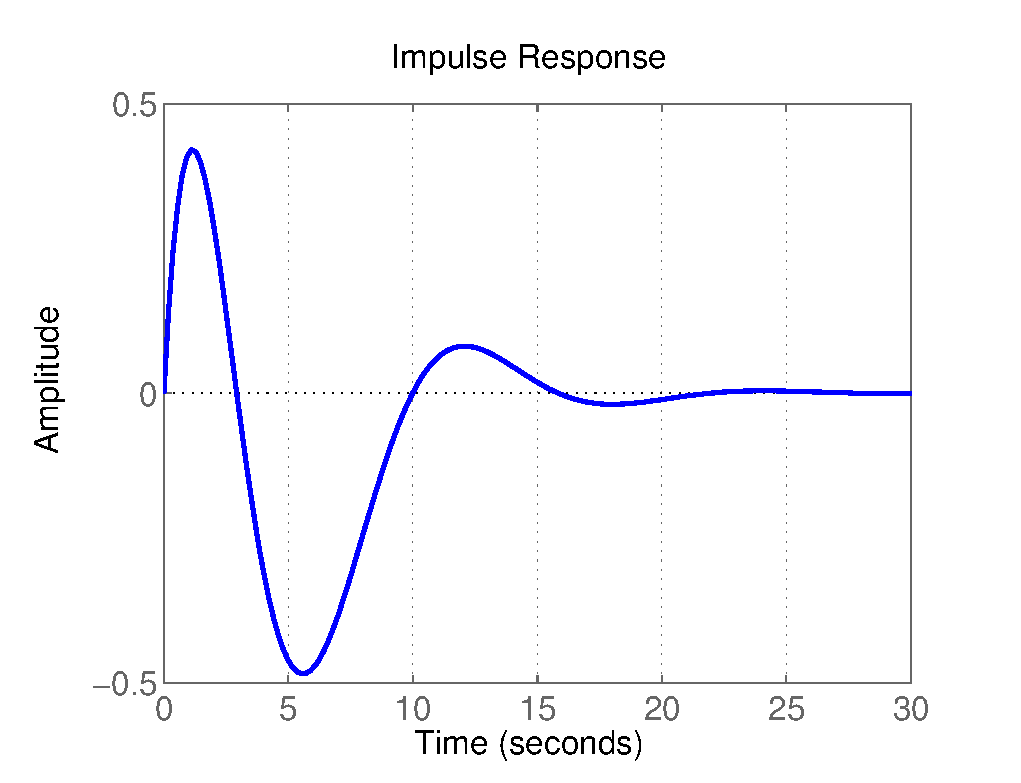
\includegraphics[width = \textwidth]{scheme/impulse}
		\caption{График весовой функции}
	\end{subfigure}
	\caption{Графики переходной и весовой функции замкнутой системы}
	\label{stepimpulse}
\end{figure}
По графику переходной функции видим, что установившееся время переходного процесса равно 17,5c. Значение перерегулирования $\sigma=\displaystyle{\frac{-1,25+1}{-1}\cdot100\%=25\%}$, затухание равно 0.

Перейдём к представлению замкнутой системы в форме В-С-В с помощью команды [A,B,C,D]=tf2ss(b,a), где b-числитель передаточной функции замкнутой системы, a-знаменатель.\par
Получим следующие матрицы:
\begin{equation*}
A =\begin{bmatrix}
    0       &   1   &   0 \\
    0       &   0   &	1 \\
    -0,16677    & -0,5833  &   -1
\end{bmatrix}
\end{equation*}
\begin{equation*}
B =\begin{bmatrix}
    0  \\
	0  \\
	1
\end{bmatrix}
\end{equation*}
\begin{equation*}
C =\begin{bmatrix}
    -0,1667 & 0,8333  & 0 \\
\end{bmatrix}
\end{equation*}

С помощью команд ctrb(A,B) и obsv(A,C) найдём соответственно матрицу управляемости и наблюдаемости.
\begin{equation*}
U_y =\begin{bmatrix}
    0   &   0   &   1 \\
    0   &   1   &	-2 \\
    1   &   -1  &   0,4167
\end{bmatrix}
\end{equation*}
\begin{equation*}
U_n =\begin{bmatrix}
    -0,1667 & 0,8333 & 0 \\
    0  & -0,1667 & 0,8333 \\
    -0,1389 & -0,4861 & -1
\end{bmatrix}
\end{equation*}\par
Так как ранг $U_y=U_n$ равен порядку системы, следовательно система является полностью управляемой и наблюдаемой.

\newpage
\begin{center}
	\section*{Вывод}
\end{center}
С помощью прикладного пакета Matlab Control System Toolbox можно достаточно быстро и точно исследовать линейную непрерывную систему любого порядка.\par
При помощи функций Matlab pole и zero, а также pzmap находятся полюса и нули передаточной функции, по которым на основе корневого критерия можно сделать вывод об устойчивости системы.\par
Воспользовавшись функциями bode и margin легко построить графики ЛАЧХ и ЛФЧХ, из которых можно найти частоту среза и запасы устойчивости системы по амплитуде и по фазе.\par
Функция nyquist строит АФЧХ системы, по которой тоже можно судить об устойчивости системы, однако следует всё же придерживаться корневого критерия устойчивости, так как критерий устойчивости Найквиста, применим относительно замкнутых систем.\par
По передаточной функции разомкнутой системы rlocus строит диаграмму расположения на комплексной плоскости нулей и полюсов замкнутой системы при изменении коэффициента отрицательной обратной связи
от 0 до $\infty$. В данном же случае система устойчива при отрицательных значениях К, поэтому на рисунке \ref{rlocus} это не отражено.\par
Построение графика переходной функции производится функцией step, а построение графика импульсной функции --- impulse. Из этих графиков можно определить время переходного процесса, значение перерегулирования, а также затухание колебаний в случае колебательных процессов.\par
В ходе исследования была получена устойчивая система, полностью управляемая и наблюдаемая, замкнутая жестко положительной обратной связью.

\end{document}
